\documentclass[oneside]{article}
 \headheight = 25pt
\footskip = 20pt
\usepackage{graphicx}

\usepackage{mdwlist}
\usepackage[T1]{fontenc}
\renewcommand{\rmdefault}{ppl}
\usepackage{fancyhdr}
 \pagestyle{fancy}
 \lhead{\textbf{\textsc{\small Scott O'Connor\\Metaphysics}}}
 \chead{}
 \rhead{\large\textbf{\textsc{Space 2}}}
 \lfoot{\footnotesize{\thepage}}
 \cfoot{}
 \rfoot{\footnotesize{\today}}
 \usepackage{longtable,booktabs}
\tolerance=700


\begin{document}
\thispagestyle{fancy}



\subsection*{Kant's Argument for Absolutism}\label{master-argument}

Recall Kant's argument strategy: there are spatial differences between right and
left hands. We want to know what gives a hand one of these spatial
features as opposed to another. The reason why a giraffe is taller than
a mouse is that the height of the former is greater than the height of
the latter. Similarly, what is it about my left hand that makes it a
left hand as opposed to a right hand? We'll identify the only viable
options for explaining handedness and exclude all but one, Absolutism.

\begin{enumerate}

\item
  A hand is left or right either (a) solely in virtue of the
  \emph{internal} relations among the parts of the hand, or (b) at least
  partly in virtue of the \emph{external} relations of the hand to other
  material objects, or (c) in virtue of the \emph{external} relations of
  the hand to space itself.
\item
  Since the internal relations are the same for right and left, a hand
  is not left or right solely in virtue of its internal relations,
\item
  A hand is neither right nor left even partly in virtue of its
  relations to other material objects.
\item
  Therefore, a hand is left or right at least party in virtue of its
  relation to absolute space.\footnote{`Incongruent Counterparts and
    Higher Dimensions', by James Van Cleve}
\end{enumerate}
1--3 state the premises of the argument. 4 states the conclusion. The
argument is valid. So if the premises are true, then 4 must also be true, i.e., if the premises are true, then absolute space exists. Here are the
arguments for the premises.

\subsection*{P2. Internalism}\label{p2.-internalism}

Internalists accept 1 and 3, but they rejects 2. They accept that a hand
that was all alone in the Universe would still be a right or left hand,
but they think that it's being left or right can be explained without
looking outside the hand itself. The features of the hand alone, they
claim, will make it a right or left one. Hence, one needs no other
material objects or space itself to explain these features. Kant raises the following objection:

\begin{enumerate}

\item[a.]
  The internal relations of both the left and right hand are distances
  between points and angles between lines, e.g., the length of the index
  finger.
\item[b.]
  The internal relations of both the left and right hand are identical.
\item[c.]
  If the internal relations of a right hand make it a right hand, then
  they cannot be identical to the internal relations of a left hand.
\item[d.]
  The internal relations of a right hand do not make it a right hand
  (similarly for the left hand)\ldots{}(from a--c)
\end{enumerate}

Our conclusion says that internal relations cannot distinguish right
from left handedness. Internalism, then, is false. 

\subsection*{P3. Externalism}\label{p3.-externalism}

Externalists accept 1 and 2, but reject 3. They claim that being a left
or right hand depends on a relationship to other material objects. Kant raises the following objection:

\begin{enumerate}

\item[a.] 
  Suppose that there is a world in which only a hand, H, exists.
\item[b.]
  Suppose that a body possessing no hands pops into existence.
\item[c.]
  H can fit only the left or the right wrist.
\item[d.]
  If H fits the right wrist, H was a right hand before the body popped
  into existence.
\item[e.]
  If H fits the left wrist, H was a left hand before the body popped
  into existence.
\item[f.]
  H was a right or left hand before the body popped into
  existence\ldots{}(from c--e)
\item[g.]
  H was a right or left hand when no other material object
  exists\ldots{}(from f)
\item[h.]
  H's being a right or left hand is not explained by its relationship to
  any other material object\ldots{}(from g)
\end{enumerate}
Our conclusion shows us that Externalism is false; we cannot explain why a hand is right or left by only appeal to relationships with other objects. 


\subsection*{Absolutism}\label{absolutism}

There were three candidates for explaining handedness; a right hand is right because of its internal relations, or because of its relationship to other physical objects, or because of its relationships to space itself. Kant argues against the first two options, and so concludes that the final option must be the correct one; absolute space must exist to explain handedness. Thus, he concludes that Absolutism is true. 

However, the existence of higher spatial dimensions may undermine Kant's argument. Our goal in this handout is to first understand what higher spatial dimensions are meant to be. We are primarily interested in how objects could move in such dimensions. We will see that allow a fourth dimension of movement means that a left hand could be turned into a right hand without changing its shape---freaky! We will then ask how the existence of such a spatial dimension affects Kant's argument.

\subsection*{A Fourth Dimension}

The concept of higher spatial dimensions may seem peculiar. The space that we experience seems to be three dimensional. The physical objects that we experience have \emph{length}, \emph{width}, and \emph{depth}. It is difficult to conceive an object which is not so extended. Try, for instance, to conceive of a two dimensional object. That also seems impossible. But why is it impossible? Is it because there really are no two or four dimensional objects? Or is it because we are limited by the type of creatures we are? 

In the novel \emph{Flatland}, we meet creatures who live in a two dimensional space, but who are completely unable to fathom that there is a third dimension. They can move in only two dimensions, e.g., they can move left and right, backwards and forwards. But the idea that an object could move up and down is completely alien to them. It would be like the object disappeared in one location and reappeared in a new location. But their inability to conceive of a third dimension--and moving in a third dimension--does not entail that there is no such dimension. Their inability is just that, an inability. 

Likewise, we cannot easily imagine a fourth spatial dimension. Neither can we imagine an object moving in a fourth dimension. We conceive of objects moving upwards or downward, left or right, backwards or forwards. These seem the only option. If a fourth dimension exist, there would be a fourth dimension within to move. This means an object could vanish before our eyes and reappear somewhere new. But perhaps we struggle to conceive a fourth dimension because of we are limited and not because there is no such thing. 

While we are unable to  visualize four dimensional objects, we can at least describe what they might be like and how they would move. Let us focus on a four dimensional cube. We will first describe its dimensions. We will do so by `building up' from a 1-dimensional figure. 

\begin{figure}[h]
  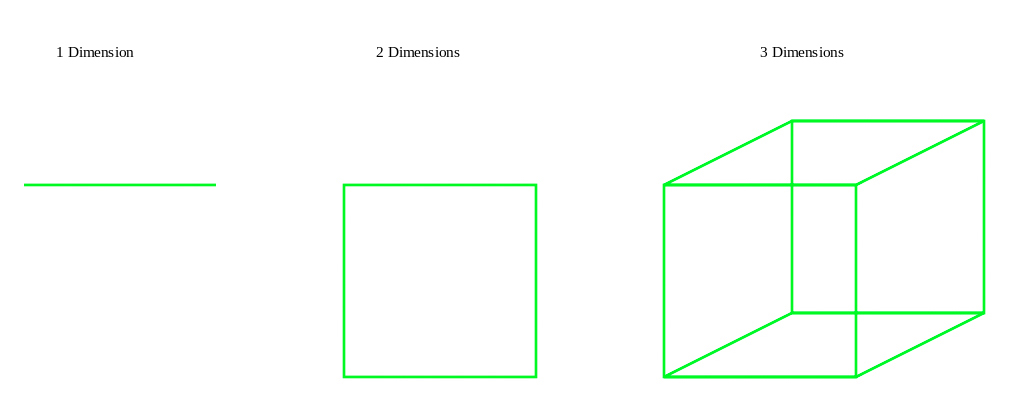
\includegraphics[width=\linewidth]{dimensions.jpg}
\end{figure}


\begin{figure}[h]
  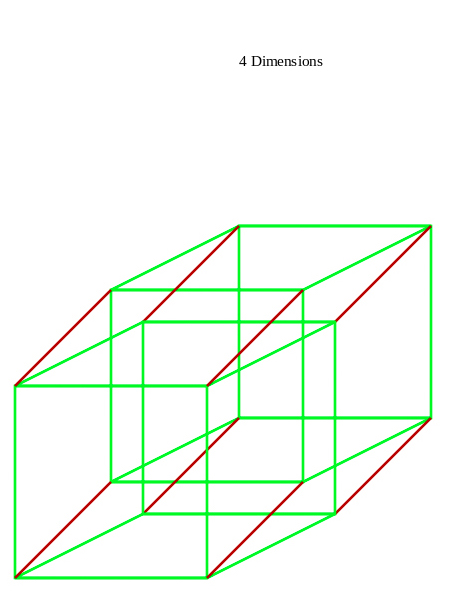
\includegraphics[width=\linewidth]{four.jpg}
\end{figure}


Dimensions

How many surfaces? 

How many points? 


Movements


\subsection*{Fourth Dimension and Incongruent Counterparts}

If higher spatial dimensions exist, then it is unclear whether there really are incongruent counterparts. Recall that we defined incongruent counterparts by saying that you cannot align such counterparts via rigid movements, movements which we assumed took place in three dimensions. You cannot turn a right hand into a left hand without changing its shape or size. I

If higher spatial dimensions exist, then it would be feasible for a right hand to be inverted and turned into a left hand, and vice versa. That appears freaky. I agree. But let us consider a two dimensional analogy. Suppose that you are looking down from above at a pair of triangles. Each triangle is red on one side and blue on the other. Now suppose you are asked to move the triangles to make them perfectly align. For them to perfectly align, their points must line up exactly and the must have the same color showing on each side, i.e., they must be both have the blue side facing up. Now suppose you can only move the triangles in two dimensions. Can you identify the two dimensional movements that will make the triangles perfectly align in the following two pictures? 


\begin{figure}[h]
  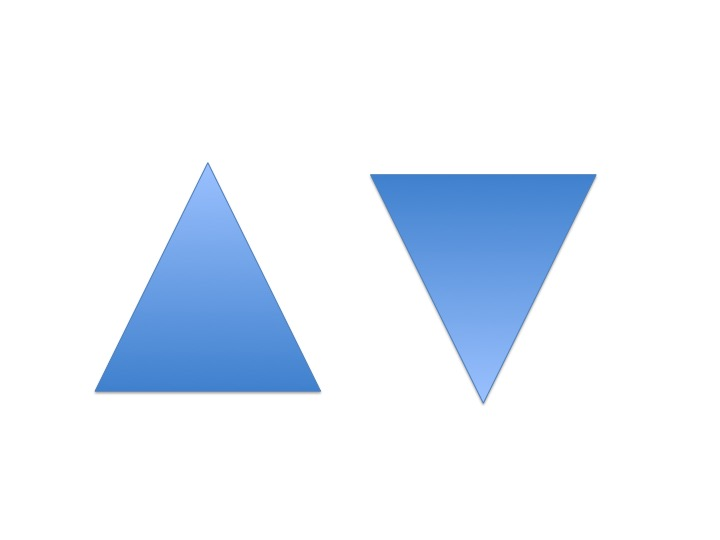
\includegraphics[width=\linewidth]{2d.jpg}
\end{figure}


\begin{figure}[h]
  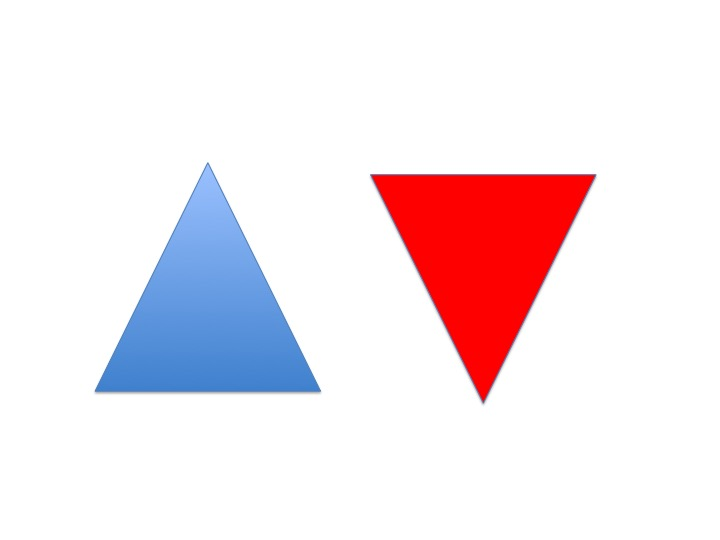
\includegraphics[width=\linewidth]{3d.jpg}
\end{figure}

It is easy to complete the task in the first picture by moving the triangle backwards or forwards, to the left or to the right. But it is impossible to complete the task with the second picture. There are no series of two dimensional movements that will make the triangles perfectly align. Their shapes may align, but the sides will never have both their blue sides facing upwards. 




\begin{figure}[h]
  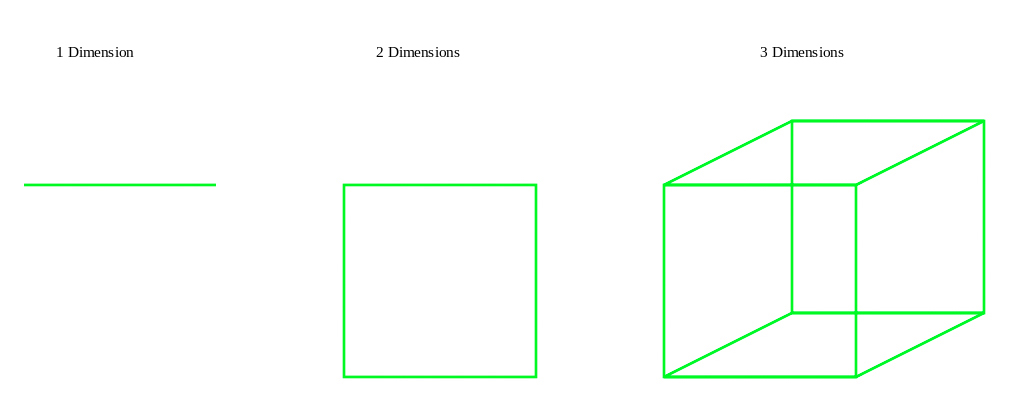
\includegraphics[width=\linewidth]{dimensions.jpg}
\end{figure}


 

\subsection{The Master Argument}

Such a possibility affects the various options Kant outlined as follows: 


\begin{description}
\item[Internalism:]  if the hands can be flipped in a fourth dimension to make them congruent, then right handedness and left handedness cannot be intrinsic properties of the  hands.
\item[Externalism:] if the hands can be flipped in a fourth dimension to make them congruent, then 
a hand does not have handedness at all if it exists all alone in the Universes. Thus, Kant's argument against Externalism fails. 
\begin{itemize}
\item Might there be four-dimensional incongruent counterparts? 
\end{itemize}
\item[Absolutism:] Kant argued for this position by eliminating Internalism and Externalism. But since the existence of a fourth spatial dimension undermines his argument for Externalism, he cannot claim to have eliminated it. 
\end{description}



https://flatland.vhx.tv/packages/flatland-the-movie/videos/flatland-vhxv2






\end{document}
